\section{Phát hiện Vật thể (Object Detection)}
\label{sec:object_detection}

Nếu phân loại ảnh là bước đầu tiên để một cỗ máy "nhận biết" thế giới, thì phát hiện vật thể là bước nhảy vọt thực sự hướng tới sự "thấu hiểu". Bài toán không còn dừng lại ở việc gán một nhãn chung cho toàn bộ bức ảnh, mà đòi hỏi mô hình phải trả lời hai câu hỏi cùng một lúc: \textbf{"Có những vật thể gì trong ảnh?" (Phân loại)} và \textbf{"Chúng đang ở đâu?" (Định vị)}.

Đầu ra của một mô hình phát hiện vật thể không phải là một nhãn duy nhất, mà là một danh sách các đối tượng được tìm thấy. Mỗi đối tượng được biểu diễn bởi:
\begin{itemize}
	\item Một \textbf{khung hộp bao (bounding box)}, thường được định nghĩa bởi tọa độ của góc trên bên trái và góc dưới bên phải $(x_{min}, y_{min}, x_{max}, y_{max})$.
	\item Một \textbf{nhãn lớp (class label)} cho đối tượng bên trong hộp (ví dụ: "chó", "mèo", "ô tô").
	\item Một \textbf{điểm số tự tin (confidence score)}, cho biết mức độ chắc chắn của mô hình về dự đoán của nó.
\end{itemize}

Lịch sử phát triển của các thuật toán phát hiện vật thể trong kỷ nguyên học sâu là một cuộc chạy đua hấp dẫn giữa hai trường phái chính:
\begin{enumerate}
	\item \textbf{Các bộ phát hiện hai giai đoạn (Two-stage detectors):} Hoạt động theo nguyên lý "nhìn kỹ". Giai đoạn đầu tiên đề xuất một tập hợp các vùng có khả năng chứa vật thể (region proposals), và giai đoạn thứ hai phân loại và tinh chỉnh các vùng đó. Chúng thường có độ chính xác cao hơn.
	\item \textbf{Các bộ phát hiện một giai đoạn (One-stage detectors):} Hoạt động theo nguyên lý "nhìn một lần". Chúng dự đoán trực tiếp vị trí và lớp của các vật thể từ ảnh đầu vào chỉ trong một lượt duy nhất, không có bước đề xuất vùng riêng biệt. Chúng thường nhanh hơn rất nhiều.
\end{enumerate}
Trong phần này, chúng ta sẽ lần theo dấu chân của cả hai trường phái này, từ những ý tưởng sơ khai đến các kiến trúc state-of-the-art ngày nay.

\subsection{Kỷ nguyên CNN: Từ R-CNN đến YOLO và SSD}
\label{subsec:cnn_based_detectors}

Sự thành công của AlexNet trong phân loại ảnh năm 2012 đã mở ra một câu hỏi cấp thiết: làm thế nào để áp dụng sức mạnh trích xuất đặc trưng của CNN cho bài toán phát hiện vật thể phức tạp hơn?

\subsubsection{Họ R-CNN: Cách tiếp cận Hai giai đoạn}
\label{subsubsec:r_cnn_family}

\paragraph{R-CNN (2014):} 
\textbf{Regions with CNN features (R-CNN)} \cite{Girshick2014} là mô hình tiên phong, đưa CNN vào phát hiện vật thể và nâng cao đáng kể độ chính xác so với các phương pháp cổ điển (HOG, DPM).

\textbf{Pipeline 3 giai đoạn rời rạc:}
\begin{enumerate}
	\item \textbf{Sinh vùng đề xuất (Region Proposal Generation):} 
	Sử dụng \textbf{Selective Search} để tạo ra $N \approx 2000$ vùng đề xuất $\{R_i\}_{i=1}^N$ trên ảnh đầu vào $I$. Mỗi $R_i$ là một hình chữ nhật có khả năng chứa vật thể.
	
	\item \textbf{Trích xuất đặc trưng CNN (CNN Feature Extraction):} 
	Mỗi vùng $R_i$ được "warped" về kích thước cố định $H \times W$ (ví dụ $227 \times 227$). Sau đó, qua CNN đã huấn luyện trước (AlexNet) để tạo vector đặc trưng:
	\[
	\mathbf{f}_i = \text{CNN}(R_i) \in \mathbb{R}^{d}, \quad d = 4096
	\]
	
	\item \textbf{Phân loại và Hồi quy bounding box:} 
	\begin{itemize}
		\item \textbf{Phân loại:} Vector $\mathbf{f}_i$ được đưa vào tập hợp các SVM tuyến tính, mỗi SVM cho một lớp $c$, dự đoán xác suất $p(c|R_i)$:
		\[
		p(c|R_i) = \sigma(\mathbf{w}_c^\top \mathbf{f}_i + b_c)
		\]
		\item \textbf{Hồi quy bounding box:} Một bộ hồi quy tuyến tính học các hệ số hiệu chỉnh $(t_x, t_y, t_w, t_h)$ để tinh chỉnh tọa độ dự đoán $(\hat{x}, \hat{y}, \hat{w}, \hat{h})$ sao cho khớp với ground-truth $(x, y, w, h)$:
		\[
		L_{\text{bbox}} = \sum_{i} \mathbf{1}_{\{c_i \ge 1\}} \sum_{j \in \{x,y,w,h\}} (t_{ij} - t^*_{ij})^2
		\]
		\item \textbf{Loss tổng thể:} Tổ hợp phân loại và hồi quy:
		\[
		\mathcal{L}_{\text{R-CNN}} = \sum_i L_{\text{cls}}(\mathbf{f}_i, c_i) + \lambda \sum_i L_{\text{bbox}}(\mathbf{f}_i, t_i^*)
		\]
	\end{itemize}
\end{enumerate}

\begin{center}
	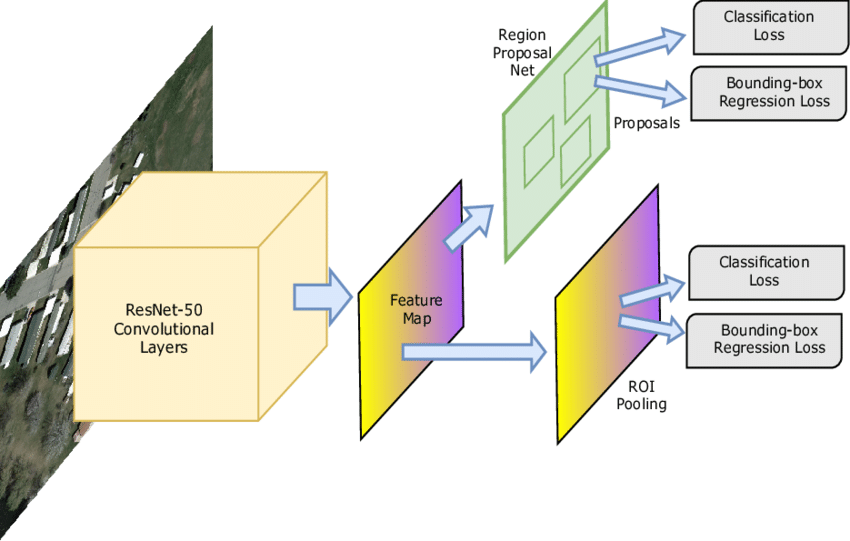
\includegraphics[width=1.0\textwidth]{images/rcnn_pipeline_diagram.png}
	\captionof{figure}{Pipeline 3 giai đoạn của R-CNN. CNN chạy trên từng vùng đề xuất, SVM phân loại, bộ hồi quy điều chỉnh bounding box.}
	\label{fig:rcnn_pipeline}
\end{center}

\textbf{Huấn luyện:} Các module (CNN, SVM, regressor) được huấn luyện rời rạc:
\begin{itemize}
	\item CNN được fine-tune trên các vùng đề xuất chứa vật thể.
	\item SVM học phân loại dựa trên feature trích xuất.
	\item Bộ hồi quy học các offsets của bounding box.
\end{itemize}

\textbf{Hạn chế:}
\begin{itemize}
	\item \textbf{Tính toán chậm:} Phải chạy CNN $N \approx 2000$ lần/ảnh, mất tới 47 giây/ảnh.
	\item \textbf{Pipeline rời rạc:} Các bước độc lập khó tối ưu hóa end-to-end.
	\item \textbf{Bộ nhớ lớn:} Trích xuất đặc trưng cho nhiều vùng đề xuất làm tăng yêu cầu bộ nhớ.
\end{itemize}

\paragraph{Fast R-CNN (2015):} 
Để giải quyết "nút thắt cổ chai" của R-CNN, Ross Girshick đề xuất \textbf{Fast R-CNN} \cite{Girshick2015}.

\textbf{Cải tiến cốt lõi:} 
Thay vì chạy CNN trên từng vùng đề xuất, Fast R-CNN chỉ chạy CNN \textbf{một lần} trên toàn bộ ảnh $I$ để tạo feature map $F$:
\[
F = \text{CNN}(I) \in \mathbb{R}^{C \times H' \times W'}
\]
Sau đó, các vùng đề xuất $\{R_i\}_{i=1}^N$ được chiếu (projected) lên feature map $F$.

\textbf{RoI Pooling:}  
Để trích xuất feature vector có kích thước cố định $d \times H_f \times W_f$ từ RoI có kích thước bất kỳ, Fast R-CNN giới thiệu \textbf{RoI Pooling}:
\begin{enumerate}
	\item Chia mỗi RoI thành một lưới $H_f \times W_f$.
	\item Áp dụng max-pooling trên mỗi ô để tạo feature map cố định:
	\[
	\mathbf{f}_i = \text{Flatten}(\text{RoI-Pool}(F, R_i)) \in \mathbb{R}^d
	\]
	\item Feature vector này được đưa vào các lớp fully-connected để phân loại và hồi quy bounding box.
\end{enumerate}

\textbf{Loss function:}  
Fast R-CNN kết hợp **phân loại đa lớp** và **hồi quy bounding box** trong một hàm loss thống nhất:
\[
\mathcal{L} = L_{\text{cls}}(p_i, c_i^*) + \lambda \mathbf{1}_{\{c_i^* \ge 1\}} L_{\text{reg}}(t_i, t_i^*)
\]
Trong đó:
\begin{itemize}
	\item $p_i$ là vector xác suất dự đoán cho các lớp, $c_i^*$ là ground-truth class.
	\item $t_i = (t_x, t_y, t_w, t_h)$ là hệ số offset dự đoán, $t_i^*$ là ground-truth offsets.
	\item $L_{\text{cls}}$ thường là cross-entropy: $L_{\text{cls}}(p_i, c_i^*) = -\log p_i[c_i^*]$.
	\item $L_{\text{reg}}$ thường là Smooth L1 loss:
	\[
	\text{SmoothL1}(x) =
	\begin{cases}
		0.5 x^2, & |x| < 1\\
		|x| - 0.5, & \text{otherwise}
	\end{cases}
	\]
\end{itemize}

\textbf{Huấn luyện end-to-end:}  
\begin{itemize}
	\item Feature map $F$ được học cùng với các lớp fully-connected cho classification và bounding box regression.
	\item RoI Pooling là phép toán bất biến với gradient, cho phép lan truyền gradient qua toàn bộ feature map.
	\item Chỉ phụ thuộc vào Selective Search để sinh vùng đề xuất, đây là bước ngoại lai chưa được học.
\end{itemize}

\begin{center}
	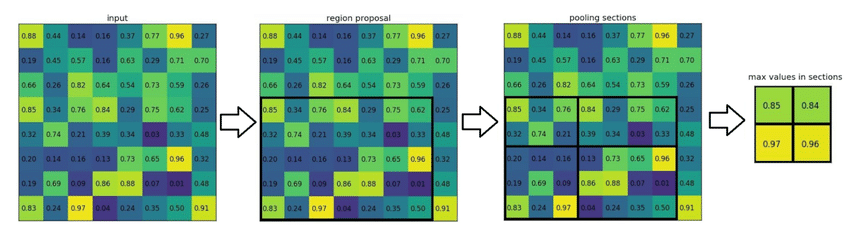
\includegraphics[width=0.8\textwidth]{images/roi_pooling_diagram.png}
	\captionof{figure}{Hoạt động của RoI Pooling. Một vùng đề xuất có kích thước bất kỳ trên feature map được chia lưới cố định và max-pooling được áp dụng.}
	\label{fig:roi_pooling}
\end{center}

\textbf{Ưu điểm so với R-CNN:}
\begin{itemize}
	\item Chạy CNN \textbf{một lần duy nhất} thay vì $N$ lần.
	\item Hỗ trợ huấn luyện \textbf{end-to-end} (trừ việc sinh vùng đề xuất).
	\item Giảm đáng kể bộ nhớ và thời gian so với R-CNN.
\end{itemize}

\textbf{Hạn chế:}  
Vẫn phụ thuộc vào Selective Search, vốn là bước chậm và không thể học được.


\paragraph{Faster R-CNN (2016):} 
"Nhanh hơn" nữa, \textbf{Faster R-CNN} \cite{Ren2015} đã giải quyết "nút thắt cổ chai" cuối cùng bằng cách loại bỏ hoàn toàn Selective Search.

\textbf{Đột phá: Mạng Đề xuất Vùng (Region Proposal Network - RPN)}  
RPN là một mạng tích chập đầy đủ (Fully Convolutional Network) trượt trên feature map $F$:
\[
F = \text{CNN}(I) \in \mathbb{R}^{C \times H' \times W'}
\]

\textbf{Anchor boxes:}  
Tại mỗi vị trí $(i,j)$ trên feature map, RPN gắn $k$ anchor boxes với các tỷ lệ (scale) và tỷ lệ khung hình (aspect ratio) khác nhau:
\[
\{a_1, a_2, \dots, a_k\} \text{ với } a_l = (x_a, y_a, w_a, h_a)
\]

RPN dự đoán cho mỗi anchor:
\begin{itemize}
	\item \textbf{Objectness score:} $p_i = P(\text{object} | a_i)$
	\item \textbf{Bounding box regression offsets:} $t_i = (t_x, t_y, t_w, t_h)$, với:
	\[
	t_x = \frac{x - x_a}{w_a},\quad t_y = \frac{y - y_a}{h_a},\quad 
	t_w = \log \frac{w}{w_a},\quad t_h = \log \frac{h}{h_a}
	\]
	Trong đó $(x,y,w,h)$ là tọa độ box ground-truth.
\end{itemize}

\textbf{Hàm loss của RPN:}  
Faster R-CNN tối ưu RPN bằng hàm loss kết hợp classification và regression:
\[
\mathcal{L}_{\text{RPN}} = \frac{1}{N_{\text{cls}}} \sum_i L_{\text{cls}}(p_i, p_i^*) + \lambda \frac{1}{N_{\text{reg}}} \sum_i p_i^* L_{\text{reg}}(t_i, t_i^*)
\]
\begin{itemize}
	\item $p_i^* \in \{0,1\}$ là nhãn objectness (1 nếu anchor có IoU với ground-truth > threshold, 0 nếu < threshold nhỏ).
	\item $L_{\text{cls}}$ là cross-entropy loss.
	\item $L_{\text{reg}}$ là Smooth L1 loss.
	\item $\lambda$ cân bằng hai thành phần loss.
\end{itemize}

\textbf{Tích hợp với Fast R-CNN:}  
Các region proposals do RPN sinh ra được chiếu lên feature map $F$ và đưa qua RoI Pooling, sau đó dùng các lớp fully-connected để:
\begin{itemize}
	\item Phân loại vật thể ($L_{\text{cls}}$)
	\item Hồi quy bounding box cuối cùng ($L_{\text{reg}}$)
\end{itemize}

\textbf{Loss toàn bộ mạng:}  
Faster R-CNN huấn luyện end-to-end với loss tổng hợp:
\[
\mathcal{L} = \mathcal{L}_{\text{RPN}} + \mathcal{L}_{\text{Fast R-CNN}}
\]

\textbf{Huấn luyện:}  
\begin{itemize}
	\item RPN và Fast R-CNN có thể huấn luyện theo hai giai đoạn hoặc đồng thời (alternating training hoặc joint training).
	\item Gradient lan truyền qua toàn bộ feature map $F$, cho phép các convolution layers học các đặc trưng tốt nhất cho cả proposal và classification.
\end{itemize}

\textbf{Ưu điểm so với Fast R-CNN:}  
\begin{itemize}
	\item Loại bỏ hoàn toàn Selective Search, tăng tốc đáng kể.
	\item Pipeline \textbf{hoàn toàn end-to-end và hợp nhất}.
	\item Cân bằng tuyệt vời giữa tốc độ (5-10 FPS) và độ chính xác.
	\item Trở thành chuẩn vàng và nền tảng cho các nghiên cứu phát hiện vật thể tiếp theo.
\end{itemize}

\paragraph{Mask R-CNN (2017):}
\textbf{Mask R-CNN} \cite{He2017} là sự mở rộng trực tiếp của Faster R-CNN, nhằm giải quyết bài toán \textbf{Instance Segmentation}, tức là vừa phát hiện bounding box, vừa phân đoạn từng đối tượng riêng biệt trong ảnh.

\textbf{Cải tiến chính:}
\begin{itemize}
	\item \textbf{Thêm nhánh Mask:} Mask R-CNN giữ nguyên Faster R-CNN để dự đoán bounding box và class, nhưng thêm một nhánh thứ ba để dự đoán mặt nạ nhị phân (binary mask) cho mỗi RoI.
	\item \textbf{RoIAlign:} Thay thế RoI Pooling bằng \textbf{RoIAlign} để tránh lỗi lượng tử hóa tọa độ khi chiếu RoI lên feature map, giúp mặt nạ dự đoán chính xác hơn.
\end{itemize}

\textbf{Hàm mất mát (Loss Function):} Mask R-CNN huấn luyện với một loss tổng hợp:
\begin{equation}
	L = L_{\text{cls}} + L_{\text{box}} + L_{\text{mask}}
\end{equation}
\begin{itemize}
	\item $L_{\text{cls}}$: Cross-entropy loss cho phân loại lớp.
	\item $L_{\text{box}}$: Smooth L1 loss cho hồi quy bounding box.
	\item $L_{\text{mask}}$: Binary cross-entropy loss trên mỗi pixel của mask.
\end{itemize}

\textbf{Tầm quan trọng:}
Mask R-CNN trở thành chuẩn mực cho các bài toán phân đoạn vật thể hiện đại. Nó kết hợp độ chính xác cao của Faster R-CNN với khả năng phân đoạn chi tiết từng đối tượng, và là nền tảng cho nhiều ứng dụng như phân đoạn y tế, tự lái, và nhận diện vật thể phức tạp.

\begin{center}
	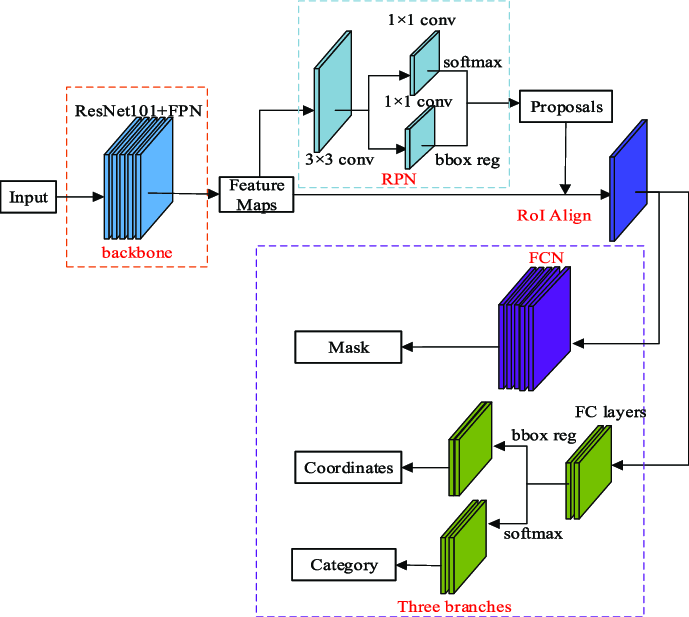
\includegraphics[width=0.95\textwidth]{images/mask_rcnn_diagram.png}
	\captionof{figure}{Kiến trúc Mask R-CNN: thêm nhánh Mask cho mỗi RoI, sử dụng RoIAlign để tăng độ chính xác của mặt nạ.}
	\label{fig:mask_rcnn}
\end{center}

\begin{mdframed}[style=infobox]
	\textbf{Các Khái niệm Cốt lõi: IoU và NMS}
	\begin{itemize}
		\item \textbf{Intersection over Union (IoU):} Là một thước đo để đánh giá mức độ trùng khớp giữa hai bounding box (ví dụ, một box dự đoán và một box ground-truth). Nó được tính bằng tỷ lệ giữa diện tích phần giao và diện tích phần hợp. Một IoU cao (ví dụ, > 0.5) cho thấy sự trùng khớp tốt.
		\begin{equation}
			\text{IoU}(A, B) = \frac{\text{Area}(A \cap B)}{\text{Area}(A \cup B)}
		\end{equation}
		\item \textbf{Non-Maximum Suppression (NMS):} Một mô hình phát hiện thường tạo ra nhiều bounding box chồng chéo cho cùng một vật thể. NMS là một thuật toán hậu xử lý để lọc bỏ các box dư thừa. Nó hoạt động bằng cách: (1) Chọn box có điểm tự tin cao nhất. (2) Loại bỏ tất cả các box khác có IoU với box đã chọn lớn hơn một ngưỡng nhất định. (3) Lặp lại quá trình cho đến khi không còn box nào để xử lý.
	\end{itemize}
\end{mdframed}

Họ R-CNN đánh dấu một bước tiến lớn trong phát hiện vật thể dựa trên CNN, bắt đầu với \textbf{R-CNN (2014)} \cite{Girshick2014}, mô hình tiên phong sử dụng pipeline 3 giai đoạn rời rạc gồm sinh vùng đề xuất bằng Selective Search, trích xuất đặc trưng CNN cho từng vùng, và phân loại kết hợp với hồi quy bounding box. R-CNN đạt độ chính xác vượt trội so với các phương pháp cổ điển nhưng rất chậm (~47 giây/ảnh) do phải chạy CNN trên từng vùng đề xuất, và khó huấn luyện end-to-end.

Tiếp theo, \textbf{Fast R-CNN (2015)} \cite{Girshick2015} cải thiện hiệu suất bằng cách chỉ chạy CNN một lần trên toàn bộ ảnh để tạo feature map, sau đó sử dụng \textbf{RoI Pooling} để trích xuất các vector đặc trưng cố định cho từng vùng đề xuất. Cải tiến này giúp Fast R-CNN nhanh hơn R-CNN hàng chục lần và cho phép huấn luyện end-to-end (ngoại trừ bước sinh vùng đề xuất), tuy nhiên vẫn phụ thuộc vào Selective Search, vốn chậm và không tối ưu.

Đến \textbf{Faster R-CNN (2016)} \cite{Ren2015}, bước cải tiến quan trọng là tích hợp trực tiếp \textbf{Mạng Đề xuất Vùng (Region Proposal Network - RPN)} vào kiến trúc chính, cho phép mạng tự học cách sinh các vùng đề xuất mà không cần Selective Search. RPN sử dụng anchor boxes với các tỷ lệ và tỷ lệ khung hình khác nhau, dự đoán đồng thời xác suất chứa vật thể (objectness) và các hệ số hiệu chỉnh vị trí. Nhờ đó, Faster R-CNN trở thành pipeline phát hiện vật thể hoàn toàn end-to-end, cân bằng giữa tốc độ (5-10 FPS) và độ chính xác, trở thành chuẩn vàng cho nhiều nghiên cứu và ứng dụng sau này.

Bài học rút ra từ họ R-CNN là việc kết hợp các ý tưởng cơ bản như trích xuất đặc trưng CNN, region proposals, và bounding box regression với các cải tiến kiến trúc như RoI Pooling và RPN, đồng thời huấn luyện end-to-end, có thể đạt được cả độ chính xác cao lẫn tốc độ hợp lý. Đây cũng là nền tảng cho nhiều bộ phát hiện một giai đoạn hiện đại như YOLO, SSD, và RetinaNet.

\begin{center}
	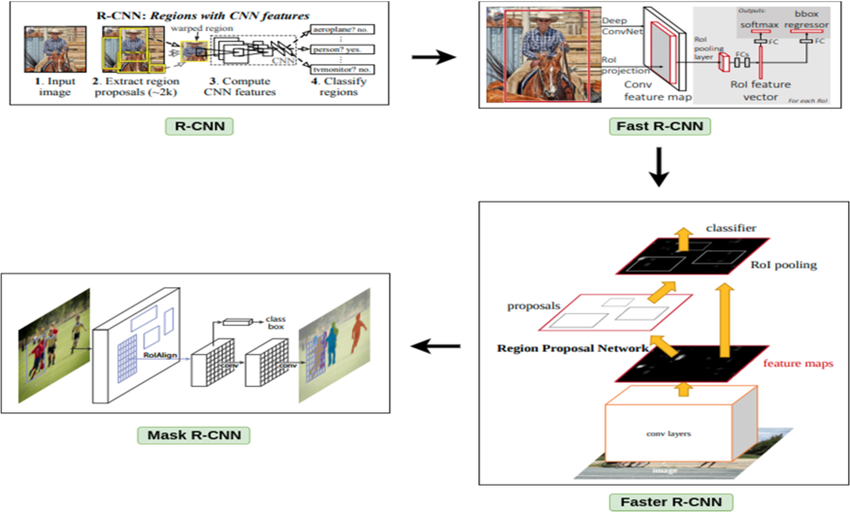
\includegraphics[width=0.95\textwidth]{images/rcnn_evolution_diagram.png}
	\captionof{figure}{Tổng quan quá trình phát triển của họ R-CNN: từ R-CNN → Fast R-CNN → Faster R-CNN. Mỗi bước cải tiến tập trung vào tăng tốc độ, đơn giản hóa pipeline, và hướng tới huấn luyện end-to-end.}
	\label{fig:rcnn_evolution}
\end{center}

\subsubsection{Các bộ phát hiện Một giai đoạn: Nhanh và Hiệu quả}
\label{subsubsec:one_stage_detectors}

\paragraph{YOLO (You Only Look Once, 2016–nay):}
Họ mô hình \textbf{YOLO} \cite{Redmon2016} của Joseph Redmon đã khởi xướng một triết lý hoàn toàn khác: coi phát hiện vật thể như một bài toán hồi quy duy nhất, end-to-end và single-shot.

\textbf{Nguyên lý cốt lõi:} Ảnh đầu vào được chia thành một lưới $S \times S$. Mỗi ô lưới dự đoán $B$ bounding box, confidence score, và xác suất các lớp của vật thể có tâm nằm trong ô đó. Tất cả dự đoán được thực hiện trong \textbf{một lần forward pass}, từ đó đạt tốc độ thời gian thực cao.

\begin{itemize}
	\item \textit{Loss function cơ bản (YOLOv1):}
	\begin{equation}
		\begin{split}
			\mathcal{L} &= \lambda_{\text{coord}} \sum_{i=0}^{S^2} \sum_{j=0}^{B} \mathbf{1}_{ij}^{\text{obj}} 
			\Big[ (x_i - \hat{x}_i)^2 + (y_i - \hat{y}_i)^2 \Big] \\
			&+ \lambda_{\text{coord}} \sum_{i=0}^{S^2} \sum_{j=0}^{B} \mathbf{1}_{ij}^{\text{obj}} 
			\Big[ (\sqrt{w_i} - \sqrt{\hat{w}_i})^2 + (\sqrt{h_i} - \sqrt{\hat{h}_i})^2 \Big] \\
			&+ \sum_{i=0}^{S^2} \sum_{j=0}^{B} \mathbf{1}_{ij}^{\text{obj}} (C_i - \hat{C}_i)^2 \\
			&+ \lambda_{\text{noobj}} \sum_{i=0}^{S^2} \sum_{j=0}^{B} \mathbf{1}_{ij}^{\text{noobj}} (C_i - \hat{C}_i)^2 \\
			&+ \sum_{i=0}^{S^2} \mathbf{1}_{i}^{\text{obj}} \sum_{c \in \text{classes}} (p_i(c) - \hat{p}_i(c))^2
		\end{split}
	\end{equation}
	
	\item \textit{Tiến hóa các phiên bản YOLO:}
	\begin{itemize}
		\item \textbf{YOLOv1 (2016):} 
		\begin{itemize}
			\item Backbone: Darknet-19, đơn giản, 19 conv + 5 max-pooling.
			\item Dự đoán trực tiếp tọa độ và class probabilities.
			\item Hạn chế: vật thể nhỏ khó detect, không dùng anchor boxes.
		\end{itemize}
		
		\item \textbf{YOLOv2 / YOLOv3 (2017–2018):} 
		\begin{itemize}
			\item Giới thiệu \textbf{anchor boxes}: dự đoán offsets, cải thiện dự đoán vật thể nhỏ và đa tỉ lệ.
			\item Multi-scale prediction: dự đoán từ nhiều feature map khác nhau.
			\item Backbone: Darknet-19 (v2), Darknet-53 (v3) với residual connections.
			\item Loss function nâng cao: GIoU hoặc CIoU thay cho MSE bounding box.
		\end{itemize}
		
		\item \textbf{YOLOv4 / YOLOv5 (2020–2021):} 
		\begin{itemize}
			\item Backbone CSPNet (Cross Stage Partial) tăng hiệu năng tính toán.
			\item Neck: PANet (Path Aggregation Network) cho multi-scale feature fusion.
			\item Augmentation mạnh: mosaic, mixup, hue-saturation-jitter, random scaling.
			\item Optimizer: AdamW, learning rate scheduler, label smoothing.
			\item Giữ balance speed–accuracy, tối ưu cho GPU.
		\end{itemize}
		
		\item \textbf{YOLOv6–v8 (2022–2024):} 
		\begin{itemize}
			\item Anchor-free hoặc dynamic anchor trong một số phiên bản.
			\item Loss function nâng cao: Varifocal Loss, CIoU/Focal Loss, cải thiện learning khi class imbalance.
			\item Edge optimization: inference nhanh (>100 FPS), tensor cores, INT8/FP16.
			\item Backbone \& Neck: Efficient CSP, attention blocks (CBAM, SPP), multi-scale prediction.
			\item End-to-end pipeline hoàn thiện, dễ triển khai trên nhiều nền tảng.
		\end{itemize}
	\end{itemize}
	
	\item \textit{Bài học rút ra:}  
	YOLO đã biến phát hiện vật thể từ bài toán nhiều giai đoạn (R-CNN) thành single-shot, end-to-end, và tiếp tục phát triển để xử lý đa dạng tỉ lệ, vật thể nhỏ, class imbalance, đồng thời tối ưu hóa cho tốc độ và hiệu năng. Đây là lý do nó trở thành chuẩn mực trong các ứng dụng thời gian thực từ YOLOv1 → YOLOv8.
\end{itemize}

\paragraph{SSD (Single Shot MultiBox Detector, 2016):} 
\textbf{SSD} \cite{Liu2016} kết hợp sự đơn giản của YOLO với ý tưởng sử dụng các đặc trưng đa tỷ lệ, mang lại sự cân bằng giữa tốc độ và độ chính xác.

\textbf{Nguyên lý cốt lõi:} SSD thực hiện dự đoán trên nhiều feature map ở các độ sâu khác nhau trong mạng:
\begin{itemize}
	\item Feature map nông (high resolution) để phát hiện vật thể nhỏ.
	\item Feature map sâu (low resolution) để phát hiện vật thể lớn.
	\item Mỗi vị trí trên feature map dự đoán nhiều bounding box với confidence score và class probabilities, dựa trên \textbf{anchor boxes} (default boxes) được thiết lập sẵn.
\end{itemize}

\begin{itemize}
	\item \textit{Loss function:} SSD sử dụng \textbf{Smooth L1 loss} cho bounding box regression và \textbf{cross-entropy loss} cho phân loại:
	\begin{equation}
		\mathcal{L}(x, c, l, g) = \frac{1}{N} \big( \mathcal{L}_{\text{conf}}(x, c) + \alpha \mathcal{L}_{\text{loc}}(x, l, g) \big)
	\end{equation}
	\begin{itemize}
		\item $x_{ij}=1$ nếu default box $i$ khớp với ground-truth $j$, ngược lại $0$.
		\item $\mathcal{L}_{\text{loc}}$: Smooth L1 loss giữa offsets dự đoán và offsets ground-truth.
		\item $\mathcal{L}_{\text{conf}}$: cross-entropy loss cho class prediction.
		\item $\alpha$: trọng số để cân bằng giữa localization và confidence.
	\end{itemize}
	
	\item \textit{Bài học rút ra:}  
	SSD cho thấy rằng bằng cách sử dụng các feature map đa tỷ lệ, kết hợp anchor boxes và dự đoán một lần (single-shot), có thể đạt được cả tốc độ thời gian thực và hiệu năng tốt, đặc biệt là đối với vật thể nhỏ. Đây là nền tảng cho nhiều phát triển sau này như RetinaNet và các phiên bản SSD cải tiến.
\end{itemize}


\paragraph{RetinaNet và Focal Loss (2017):}  
Một trong những thách thức lớn nhất của các bộ phát hiện một giai đoạn là \textbf{mất cân bằng cực độ giữa các lớp}. Trong một ảnh, số lượng anchor hoặc vị trí nền (background) lớn hơn rất nhiều so với các vị trí chứa vật thể (foreground), làm hàm mất mát bị chi phối bởi các mẫu nền dễ phân loại.

\textbf{Kiến trúc RetinaNet:}  
\begin{itemize}
	\item Backbone: ResNet (với FPN – Feature Pyramid Network) để trích xuất đặc trưng đa tỷ lệ.
	\item Head: hai nhánh riêng biệt cho \textbf{classification} và \textbf{bounding box regression}.
	\item Anchor boxes: được đặt trên các feature map đa tỷ lệ, với nhiều tỉ lệ (aspect ratio) và kích thước.
\end{itemize}

\textbf{Focal Loss:} Giải quyết imbalance bằng cách "tập trung" vào các mẫu khó:  
\begin{equation}
	\text{FL}(p_t) = -\alpha_t (1 - p_t)^\gamma \log(p_t)
\end{equation}
\begin{itemize}
	\item $p_t$: xác suất dự đoán đúng của mẫu.  
	\item $\alpha_t$: trọng số cân bằng giữa các lớp.  
	\item $\gamma$: hyperparameter để giảm trọng số các mẫu dễ phân loại.  
\end{itemize}
\textit{Trực giác:}  
\begin{itemize}
	\item Mẫu dễ ($p_t \to 1$) → hệ số $(1-p_t)^\gamma \to 0$, giảm đóng góp vào loss.  
	\item Mẫu khó ($p_t \to 0$) → hệ số ≈ 1, giữ nguyên đóng góp.  
\end{itemize}

\textit{Bài học rút ra:}  
Focal Loss cho phép các bộ phát hiện một giai đoạn như RetinaNet vượt qua độ chính xác của các phương pháp hai giai đoạn (Faster R-CNN), đồng thời duy trì tốc độ inference cao. Đây là bước tiến quan trọng giúp single-shot detectors trở nên cạnh tranh về độ chính xác.

\subsection{Kỷ nguyên Transformer: DETR và các Cải tiến}
\label{subsec:transformer_based_detectors}

Năm 2020, Facebook AI Research giới thiệu một ý tưởng táo bạo: loại bỏ hoàn toàn các thành phần thủ công như anchor, RPN, và NMS. Kết quả là \textbf{DEtection TRansformer (DETR)} \cite{Carion2020}.

\paragraph{Kiến trúc và Nguyên lý:}  
DETR kết hợp CNN backbone với Transformer để thực hiện phát hiện vật thể end-to-end:
\begin{enumerate}
	\item \textbf{Backbone CNN:} Trích xuất feature map 2D từ ảnh đầu vào (ví dụ: ResNet-50/101).
	\item \textbf{Transformer Encoder-Decoder:}
	\begin{itemize}
		\item Feature map được "dát phẳng" thành chuỗi token, bổ sung positional encoding, và đưa vào \textbf{Encoder}. Self-attention của encoder giúp feature mỗi vị trí chứa thông tin bối cảnh toàn cục.
		\item \textbf{Object Queries:} Một tập vector có thể học được (ví dụ 100 queries) được đưa vào \textbf{Decoder}. Mỗi query học cách tập trung vào một đối tượng cụ thể thông qua cross-attention giữa query và output của encoder.
	\end{itemize}
	\item \textbf{Prediction Heads:} Output của mỗi query được đưa qua một FFN nhỏ để dự đoán trực tiếp bounding box (x, y, w, h) và class.
\end{enumerate}

\begin{center}
	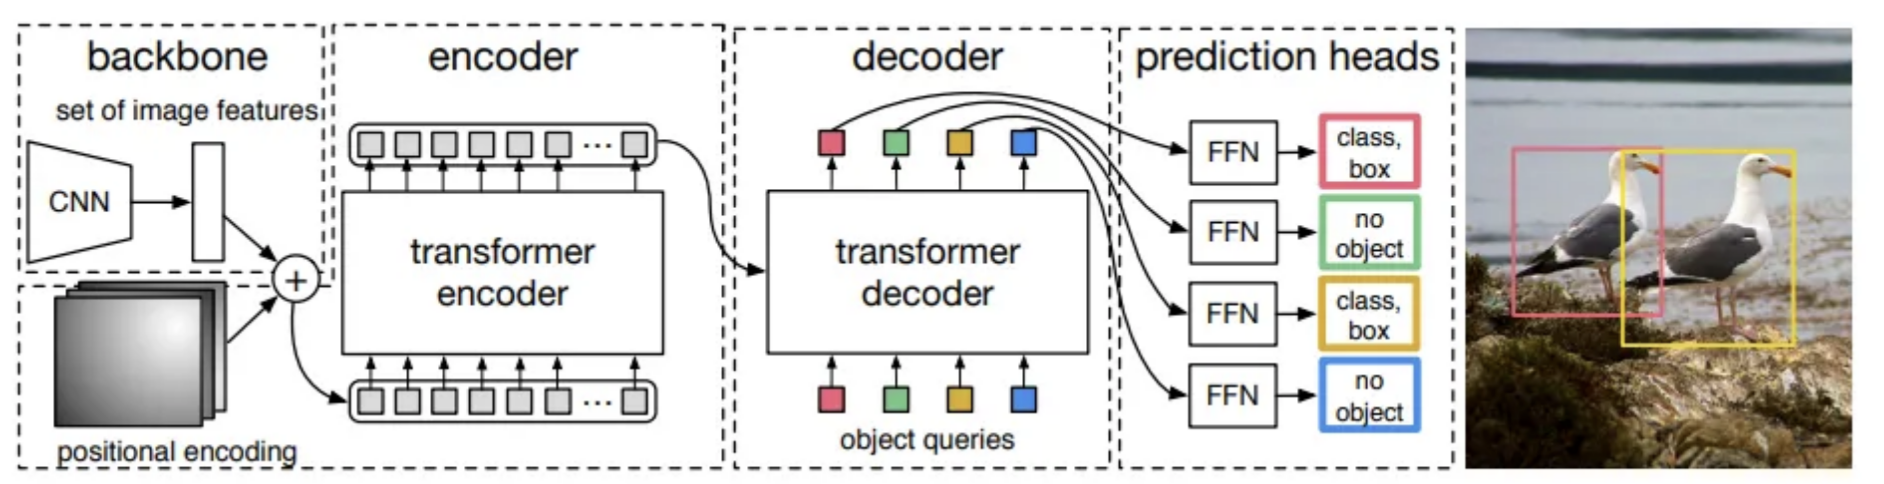
\includegraphics[width=1.0\textwidth]{images/detr_architecture_diagram.png}
	\captionof{figure}{Sơ đồ kiến trúc DETR: CNN backbone + Transformer Encoder-Decoder + object queries. Mỗi query dự đoán trực tiếp một đối tượng.}
	\label{fig:detr_architecture}
\end{center}

\paragraph{Đột phá:}  
\begin{itemize}
	\item Pipeline \textbf{end-to-end} thực sự, không cần anchor, RPN hay NMS.
	\item Sử dụng \textbf{Hungarian bipartite matching loss} để gán một-một giữa dự đoán và ground-truth.
	\item Mỗi object query học cách dự đoán một đối tượng, độc lập với các heuristic truyền thống.
\end{itemize}

\paragraph{Hạn chế ban đầu:}  
\begin{itemize}
	\item Hội tụ chậm, cần training nhiều epoch.
	\item Hiệu quả thấp trên vật thể nhỏ do attention toàn cục trên feature map thô.
\end{itemize}

\paragraph{Cải tiến sau này:}  
\begin{itemize}
	\item \textbf{Deformable DETR:} Giới thiệu attention tập trung vào các điểm tham chiếu nhỏ, cải thiện tốc độ hội tụ và hiệu quả với vật thể nhỏ.
	\item \textbf{DINO, DN-DETR:} Sử dụng denoising queries và dynamic anchor query, tăng tốc độ hội tụ và nâng cao độ chính xác.
	\item Kết hợp multi-scale feature map, cải thiện phát hiện đa tỷ lệ.
\end{itemize}

\paragraph{Bài học rút ra:}  
DETR và các biến thể chứng minh rằng \textbf{transformer có thể thay thế hoàn toàn các thành phần heuristic trong detection}, mở ra một kỷ nguyên mới của các bộ phát hiện end-to-end, đơn giản nhưng mạnh mẽ, đặc biệt khi kết hợp với các cơ chế attention hiệu quả và multi-scale feature.


\subsection{YOLO Thế hệ Mới và Các Hướng đi Tiên phong}
\label{subsec:new_generation_yolo}

Cuộc đua trong phát hiện vật thể vẫn tiếp tục sôi động, với những ý tưởng mới không ngừng được đề xuất:

\begin{itemize}
	\item \textbf{YOLO-NAS (2023):} 
	\begin{itemize}
		\item Áp dụng \textbf{Neural Architecture Search (NAS)} để tự động tìm ra kiến trúc backbone tối ưu.
		\item Tối ưu hóa đồng thời \textbf{độ chính xác và tốc độ inference}, giảm sự phụ thuộc vào thiết kế thủ công.
		\item Cho phép tạo ra các phiên bản nhẹ (lightweight) hoặc mạnh (high-performance) tùy theo mục tiêu triển khai: edge device, GPU hay server.
	\end{itemize}
	
	\item \textbf{YOLO-World (2024):} 
	\begin{itemize}
		\item Kết hợp YOLO với các biểu diễn ngôn ngữ từ mô hình nền tảng \textbf{CLIP}, tạo khả năng \textbf{Open-Vocabulary Detection}.
		\item Có thể phát hiện các vật thể được mô tả bằng ngôn ngữ tự nhiên, kể cả khi chưa từng xuất hiện trong dữ liệu huấn luyện.
		\item Mở ra hướng phát triển \textbf{universal detector} có thể áp dụng trong các tình huống thực tế phức tạp, ví dụ giám sát, robot, và AR/VR.
	\end{itemize}
	
	\item \textbf{Xu hướng chung:} 
	\begin{itemize}
		\item \textbf{Kết hợp học sâu với biểu diễn đa dạng:} Ngôn ngữ, hình ảnh, ngữ cảnh.
		\item \textbf{Tối ưu inference và năng lượng:} Hỗ trợ deployment trên edge devices, sử dụng INT8/FP16, tensor cores.
		\item \textbf{Phát triển hướng generalization:} Phát hiện vật thể không giới hạn tập lớp huấn luyện, mở rộng khả năng ứng dụng trong thế giới thực.
	\end{itemize}
\end{itemize}

\paragraph{Bài học rút ra:}  
YOLO thế hệ mới cho thấy xu hướng phát triển trong detection là \textbf{tự động hóa thiết kế mạng, kết hợp đa dạng biểu diễn, và tối ưu hóa end-to-end}. Các hướng đi như Open-Vocabulary Detection hứa hẹn sẽ làm thay đổi cách các mô hình nhận thức môi trường, từ các tác vụ truyền thống sang những ứng dụng mở rộng, linh hoạt hơn trong đời sống thực.


\subsection{Các Kiến trúc Nhận biết Góc quay và Anchor-Free}
\label{subsec:angle_aware_anchor_free}

\begin{description}
	\item[Phát hiện Vật thể có Góc quay (Rotated Object Detection):] 
	Trong nhiều ứng dụng thực tế như ảnh viễn thám, OCR, hay robot gắp hàng, các vật thể thường không nằm thẳng hàng với trục của ảnh. Thay vì dùng bounding box trục-aligned truyền thống $(x, y, w, h)$, các kiến trúc này dự đoán một bounding box có 5 tham số $(x, y, w, h, \theta)$:
	\begin{itemize}
		\item $\theta$: góc quay của vật thể so với trục x.
		\item Giúp bao quanh đối tượng một cách chặt chẽ hơn, cải thiện IoU và độ chính xác cho vật thể nghiêng hoặc dài.
		\item Thường kết hợp với anchor-based hoặc anchor-free approaches, tùy kiến trúc.
	\end{itemize}
	
	\item[Anchor-based vs. Anchor-free:] 
	Cuộc tranh luận về việc có nên sử dụng "khung neo" hay không vẫn tiếp diễn.
	\begin{itemize}
		\item \textbf{Anchor-based (ví dụ: Faster R-CNN, YOLOv3):} 
		\begin{itemize}
			\item Sử dụng một tập hợp các anchor box được định nghĩa trước với nhiều scale và aspect ratio.
			\item Ưu điểm: huấn luyện ổn định, dễ hội tụ; đã chứng minh hiệu quả trong các mô hình truyền thống.
			\item Nhược điểm: cần tinh chỉnh nhiều siêu tham số, tạo ra nhiều box dư thừa, ảnh hưởng tốc độ inference.
		\end{itemize}
		\item \textbf{Anchor-free (ví dụ: FCOS, CenterNet, YOLOX):} 
		\begin{itemize}
			\item Dự đoán trực tiếp các điểm chính (như tâm, góc, kích thước) của vật thể mà không dựa vào anchor box.
			\item Ưu điểm: thiết kế đơn giản, thường nhanh hơn, dễ mở rộng sang các bài toán rotated detection.
			\item Nhược điểm: đôi khi cần loss function tinh vi hơn và sampling strategy để học tốt các vật thể nhỏ hoặc hiếm.
			\item Xu hướng hiện nay: anchor-free đang trở thành tiêu chuẩn trong nhiều bộ phát hiện hiện đại, đặc biệt cho các phiên bản YOLOv6–v8 hoặc các mô hình lightweight.
		\end{itemize}
	\end{itemize}
\end{description}

\paragraph{Ứng dụng thực tế:}  
Các kiến trúc rotated và anchor-free cực kỳ hữu ích trong giám sát hàng không (aerial imagery), nhận diện biển báo, OCR, và robot tự động, nơi các vật thể thường xuất hiện với nhiều góc quay khác nhau và cần inference nhanh.


\section*{Tài liệu tham khảo}
\begin{itemize}
	\item[1] Girshick, R., Donahue, J., Darrell, T., \& Malik, J. (2014). Rich feature hierarchies for accurate object detection and semantic segmentation. In \textit{CVPR}. (Paper gốc về R-CNN).
	\item[2] Girshick, R. (2015). Fast r-cnn. In \textit{ICCV}. (Paper gốc về Fast R-CNN).
	\item[3] Ren, S., He, K., Girshick, R., \& Sun, J. (2015). Faster r-cnn: Towards real-time object detection with region proposal networks. In \textit{NeurIPS}. (Paper gốc về Faster R-CNN và RPN).
	\item[4] Redmon, J., Divvala, S., Girshick, R., \& Farhadi, A. (2016). You only look once: Unified, real-time object detection. In \textit{CVPR}. (Paper gốc về YOLOv1).
	\item[5] Liu, W., Anguelov, D., Erhan, D., Szegedy, C., Reed, S., Fu, C. Y., \& Berg, A. C. (2016). Ssd: Single shot multibox detector. In \textit{ECCV}. (Paper gốc về SSD).
	\item[6] Lin, T. Y., Goyal, P., Girshick, R., He, K., \& Dollár, P. (2017). Focal loss for dense object detection. In \textit{ICCV}. (Paper gốc về RetinaNet và Focal Loss).
	\item[7] Carion, N., Massa, F., Synnaeve, G., Usunier, N., Kirillov, A., \& Zagoruyko, S. (2020). End-to-end object detection with transformers. In \textit{ECCV}. (Paper gốc về DETR).
	\item[8] Jocher, G., Chaurasia, A., \& Qiu, J. (2023). YOLO by Ultralytics. \textit{https://github.com/ultralytics/yolov5}. (Một trong những phiên bản YOLO hiện đại, phổ biến).
	\item[9] Cheng, T., et al. (2024). YOLO-World: Real-Time Open-Vocabulary Object Detection. \textit{arXiv preprint arXiv:2401.17270}. (Paper gốc về YOLO-World).
\end{itemize}
